\subsection{Das elektrische Strahlungsfeld}
\begin{itemize}[label={$\to$}]
\item experimentelle Beobachtungen: Licht/elektro magnetische Strahlung ausgesandt von Sternen
\item während 1000-en von Jahren die \underline{einzige} Infomationsquelle\\
\begin{tikzpicture}
\draw (0,0)circle(1 cm);
\draw[xshift=0.3 cm,yshift=0.5 cm] (-0.2,-0.4)--(0.3,-0.4)--(0.3,0.1)--(-0.2,0.1)--cycle;
\draw[->] (0.35,0.3)--(1,1.5);
\draw[->] (0.35,0.3)--(1.2,0.6)node[midway,below]{$\vec{n}$};
\draw (0.35,0.3)--(2,0.6)(0.35,0.3)--(2,1.3)(2,0.6)--(2,1.3)--(2.7,1.3)--(2.7,0.6)--(2,0.6);
\node at (2.35,0.95){$d\omega$};
\draw (0.35,0.1)--(2,-0.5)node[right]{$dA$};
\coordinate (A) at (1,1.5);
\coordinate (B) at (0.35,0.3);
\coordinate (C) at (1.2,0.6);
\pic[draw,angle eccentricity=3] {angle=C--B--A};
\node[above right] at (0.7,0.6){$\theta$};
\node[right] at (3,1){$d\omega $: Infinitesimales Raumwinkelelement};
\end{tikzpicture}\\
$dA\cos(\theta)\hat{=}$ in Richtung der einfallenden Strahlung projezierte Fläche
\item \underline{spezifische Intensität} $I_\nu$ (=spektrale Strahlungsdichte):
\begin{align*}
dE&=I_\nu dA\cos(\theta)dtd\omega d\nu\\
\nu &= \text{ Frequenz der Strahlung}\\
E &= \text{ emittierte Energie}\\
I_\nu &\text{ entspricht der Flächenhelligkeit einer (kosmischen) Quelle}\\
[I_\nu]&=\frac{\text{erg}}{\si{\cm^2\hertz\text{ ster }\s}} \quad (1 \text{erg}=\num{10}^{-7}\ \si{\J})
\end{align*}
\item spezifischer Nettofluss:
\begin{align*}
F_\nu = \int\limits_{\Omega}d\omega I_\nu\cos(\theta)\quad ,[F_\nu]=\frac{\text{erg}}{\si{cm^2\hertz\s}}
\end{align*}
der durch das Flächenelement strömt. Typischerweise (kosmologische Quellen) $\Omega << 1\ \Rightarrow \cos(\theta)\approx 1$ (in diesem Zusammenhang wird $F_\nu$ mit $S_\nu$ bezeichnet)
\item \underline{mittlere spezifische Intensität}
\begin{align*}
J_\nu&=\frac{1}{4\pi}\int d\omega I_\nu \quad , \text{Mittelwert von } I_\nu \text{über alle Winkel}\\
&\text{bei isotropem Strahlungsfeld: } J_\nu=I_\nu
\end{align*}
\item \underline{spezifische Energiedichte}:
\begin{align*}
u_\nu &= \frac{4\pi}{c}J_\nu \qquad [u_\nu]=\frac{\text{erg}}{\si{\cm^3\hertz}}\\
\text{Energie des Strahlungsfeldes}&\text{ pro Volumenelement und Frequenzintervall}
\end{align*}
\item \underline{Gesamtenergiedichte der Strahlung}: $u=\int\limits_0^\infty d\nu u_\nu$
\end{itemize}
\subsection{Strahlungstransport}
$I_\nu=\text{const.}$ entlang der Ausbreitungsrichtung eines Lichtstrahls (falls keine Emissions- oder Absorptionsprozesse stattfinden)\\
$s=$ Länge entlang des Strahls\\
$\Rightarrow \frac{dI_\nu}{ds}=\sigma \ \Rightarrow $ Flächenhelligkeit einer Quelle ist \underline{unabhängig} von ihrer Entfernung.\\
Aber: Der beobachtbare Fluss einer Quelle hängt von ihrer Entfernung $D$ ab, weil der von der Quelle eingenommene Raumwinkel abnimmt: $F_\nu \propto\frac{1}{D^2}$
\begin{itemize}[label={$\to$}]
\item inklusive Emission \& Absorption (bzw. Streuung von Licht)
\begin{align*}
\frac{dI_\nu}{ds}=-\underset{\underset{\underset{\underset{[\kappa_\nu]=\frac{1}{\si{\cm}}}{\kappa_\nu: \text{Absorptionskoeffizient}}}{\text{Absorption}}}{\uparrow}}{\kappa_\nu}\cdot I_\nu +\underset{\underset{\underset{\underset{[j_\nu]=\frac{\text{erg}}{\si{\cm^3\s\hertz}\ \text{ster}}}{\text{Emissionskoeffizient}}}{\text{Emission}}}{\uparrow}}{j_\nu} \qquad (\ast)\quad (\text{Strahlungstransportgleichung})
\end{align*}
Absorption/Emission=echte Absorption/Emission + Streuung
\item optische Tiefe $\tau_\nu(s):=\int\limits_{s_0}^s ds \kappa_\nu (s')$
\begin{align*}
\Rightarrow d\tau_\nu &=\kappa_\nu\cdot ds, s_0: \text{ Referenzpunkt auf dem Lichtstrahl}\\
(\ast)\Rightarrow \frac{dI_\nu}{d\tau_\nu}&=-I_\nu +\mathcal{S}_\nu\qquad (\ast\ast)\\
\text{wobei: } \mathcal{S}_\nu&=\frac{j_\nu}{\kappa_\nu} \quad \text{\underline{Quellfunktion}}
\end{align*}
\item formale Lösung von ($\ast\ast$):
\begin{equation*}
I_\nu(\tau_\nu)=\underset{\underset{\text{aufgrund von Absorption}}{\text{Abfall der Intensität}}}{I_\nu(0)e^{-\tau_\nu}}+\underset{\underset{\underset{\text{darauffolgender Absorption}}{\text{Emission (inklusive}}}{\text{Energiegewinn durch}}}{\int\limits_0^{\tau_\nu}d\tau_\nu'e^{\tau_\nu'-\tau_\nu}\mathcal{S}_\nu(\tau_\nu')}
\end{equation*}
formale Lösung, weil Zustand der Materie (von der $\kappa_\nu$ und $j_\nu$ abhängen) vom Strahungsfeld selbst abhängt.
\end{itemize}
\subsection{Schwarzkörperstrahlung}
\begin{itemize}[label={$\to$}]
\item Für Materie im thermischen Gleichgewicht:
\begin{align*}
\mathcal{S}_\nu&=B_\nu(T)\\
\Leftrightarrow j_\nu &=B_\nu(T)\cdot\kappa_\nu\\
\text{\underline{Kirchhoff}}&\text{\underline{sches Gesetz}}
\end{align*}
hängt nur von der Temperatur ab (und nicht von $I_\nu$!) und der Zusammensetzung der Materie
\begin{align*}
\Rightarrow I_\nu (\tau)&=I_\nu(0)e^{-\tau_\nu}+B_\nu (T)\cdot\int\limits_0^{\tau_\nu}d\tau_\nu'e^{(\tau_\nu'-\tau_\nu)}\\
&=I_\nu(0)e^{-\tau_\nu}+B_\nu(T)\cdot(1-e^{-\tau_\nu})
\end{align*}
Für größere $\tau_\nu$ gilt: $I_\nu\approx B_\nu(T)$\\
Die Strahlung der Materie im thermischen Gleichgewicht wird durch die Funktion $B_\nu(T)$ beschrieben, wenn die optische Tiefe genügend groß ist.\\
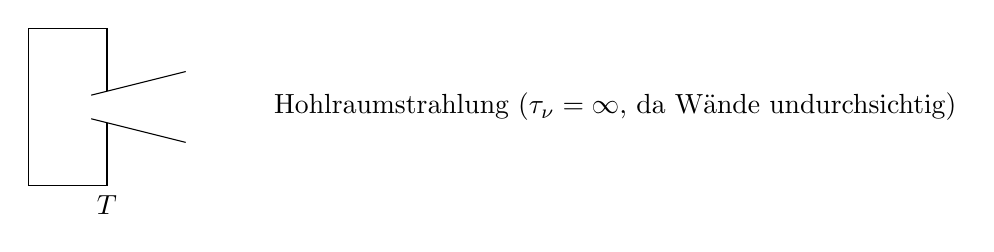
\begin{tikzpicture}
\draw (1,0.8)--(1,0)node[below]{$T$}--(0,0)--(0,2)--(1,2)--(1,1.2);
\draw (0.8,0.85)--(2,-0.05/0.2*1.2+0.85)(0.8,1.15)--(2,0.05/0.2*1.2+1.15);
\node[right] at (3,1){Hohlraumstrahlung ($\tau_\nu =\infty$, da Wände undurchsichtig)};
\end{tikzpicture}
\begin{equation*}
B_\nu(T)=\frac{2h\nu^3}{c^2}\cdot\frac{1}{e^{\frac{h\nu}{k_bT}}-1}
\end{equation*}
mit:\\
$h=\SI{6.626e-27}{\text{erg}\cdot\s}$ Plank'sches Wirkungsquantum\\
$k_B=\SI{1.38e-16}{\frac{\text{erg}}{\K}}$ Boltzmann-Konstante\\
Schwarzkörperstrahlung: 
\begin{equation*}
(\ast\ast) \Rightarrow \text{falls } \tau_\nu\to\infty \text{ gilt } I_\nu=\mathcal{S}_\nu \begin{cases} I_\nu=B_\nu(T) \\ \text{thermische Strahlung: } \mathcal{S}_\nu=B_\nu(T)\end{cases}
\end{equation*}
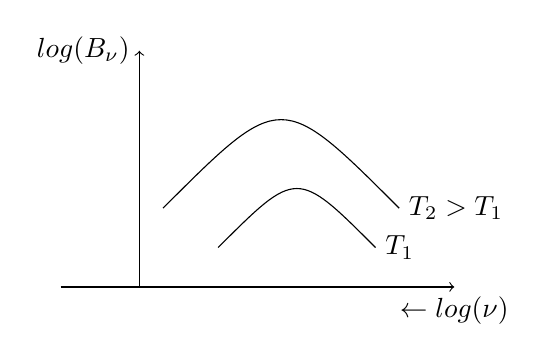
\begin{tikzpicture}
\draw[->] (-1,0)--(4,0)node[below]{$\leftarrow \text{log}(\nu)$};
\draw[->] (0,0)--(0,3)node[left]{$\text{log}(B_\nu)$};
\draw (1,0.5) .. controls +(1,1) and +(-1,1) .. (3,0.5)node[right]{$T_1$};
\draw[xshift=-0.2 cm] (0.5,1) .. controls +(1.5,1.5) and +(-1.5,1.5) .. (3.5,1)node[right]{$T_2>T_1$};
\end{tikzpicture}
\item Maximum von $B_\nu$ bei $\frac{h\nu_{max}}{k_BT}=2.82$ (Wien'sches Verschiebungsgesetz)
\underline{NB}: $\nu_{max}\approx T \ \Rightarrow$ Messung der Temperatur
\item Wg. $B_\lambda(T)d\lambda =B_\nu(T)d\nu$ mit $\lambda=\frac{c}{\nu}$
\begin{equation*}
\Rightarrow B_\lambda (T)=\frac{2hc^2}{\lambda^5}\frac{1}{e^{\frac{hc}{k_B\lambda T}}-1}
\end{equation*}
Rayleigh-Jeans-Näherung (ergibt sich bereits aus klassischer Elektrodynamik):
\begin{equation*}
B_\nu (T)\underset{\frac{h\nu}{k_BT}<<1}{\approx} \frac{2}{c^5}\nu^2k_BT
\end{equation*}
Wien-Näherung: 
\begin{equation*}
B_\nu(T)\underset{\frac{h\nu}{k_BT}>>1}{\approx} \frac{2h\nu^3}{c^2}e^{-\frac{h\nu}{k_BT}}
\end{equation*}
\item Energiedichte:
\begin{equation*}
u=\frac{4\pi}{c}\int\limits_0^\infty d\nu B_\nu(T)=\underset{\approx \num{7.56e-15}\si{\frac{\text{erg}}{\cm^3\K^4}}}{\underbrace{\frac{8\pi^5k_B^4}{15c^3h^3}}}\cdot T^4
\end{equation*}
$\Rightarrow $ Fluss, der von der Oberfläche eines schwarzen Körpers ausgeht:
\begin{align*}
F=\int\limits_0^\infty d_\nu F_\nu&=\Pi\int\limits_0^\infty d\nu B_\nu(T)\\
&=\sigma\cdot T^4 \text{ mit } \sigma=cnst\\
\sigma &= \frac{2\pi^5k_B^4}{15c^2h^3}=cnst \qquad (\text{Stefan-Boltzmann-Konstante})
\end{align*}
\end{itemize}
\subsection{Das Magnitudensystem}
\begin{itemize}[label={$\to$}]
	\item die \underline{scheinbare Helligkeit}, die das Auge wahrnimmt, verhält sich in etwa logarithmisch mit dem Strahlungsstrom (vgl. Gehörsinn, Einheit Dezibel)
		\begin{itemize}[label={$\Rightarrow$}]
			\item seit der Antike Einteilung von Sternen in \underline{Größenklassen} (qualitativ)
			\item Einführung eines quantitativen (relativen) Maysystems
		\end{itemize}
	\item[\underline{Definition}] Für zwei Quellen, die die Flüsse $S_1$ und $S_2$ haben, verhalten sich die \underline{scheinbaren Magnituden}/\underline{scheinbaren Helligkeiten} der beiden Quellen $m_1$ und $m_2$ wie:
		\begin{align*}
			m_1-m_2&=-\num{2.5}\log\left(\frac{S_1}{S_2}\right)\\
			\Leftrightarrow \frac{S_1}{S_2}&=10^{-\num{0.4}(m_1-m_2)}
		\end{align*}
	\item NB:
		\begin{equation*}
			\underset{\underset{m_2=0}{\text{z.B.} m_1=1}}{\delta m=1} \Rightarrow \frac{S_1}{S_2}\approx \num{0.4} \Leftrightarrow \frac{S_2}{S_1}=\num{2.5}\Rightarrow S_2>S_1
		\end{equation*}
	\item je größer die scheinbare Helligkeit, desto schwächer (!) die Quelle.\\
		traditionelle Referenz: Wega $m=0 \ mag$\\
		heute "'Polsequenz"' $\Rightarrow \ m^{\text{Wega}}=\num{0.03} \ mag$
		\clearpage
	\item Beispiele:
		\begin{itemize}[label={}]
			\item Sonne: $-\num{26.73}\ \si{mag}$
			\item Vollmond: $-\num{12.73}\ \si{mag}$
			\item Sirius: $-\num{1.46}\ \si{mag}$
			\item Polarstern: $\num{1.97}\ \si{mag}$
			\item Uranus: $\num{5.5}\ \si{mag}$
			\item Pluto: $\num{13.9}\ \si{mag}$
		\end{itemize}
\end{itemize}
\subsection{Farben \& absolute Helligkeit}
\begin{itemize}[label={$\to$}]
	\item Sterne haben verschiedene Farben (besser mit (z. B.) Feldstecher zu beobachten)
	\item man misst die scheinbaren Magnituden für verschiedene wohldefinierte Frequenzen (mit Hilfe von Filtersystemen, die zur Beobachtung genutzt werden) und schreibt:
		\begin{itemize}
			\item[ultraviolett] $U=m_U$
			\item[blau] $B=m_B$
			\item[sichtbar] $V=m_V$
			\item[rot] $R=m_R$
			\item[infrarot] $I=m_I$
			\item[] etc.
		\end{itemize}
		Es existieren mehrer Filtersysteme $\Rightarrow $ verschiedene gebräuchliche Magnitudendefinitionen \& Referenzpunkte
	\item \underline{Absolute Helligkeit}:
		\begin{itemize}[label={$\bullet$}]
			\item Sei $L_\nu$ die spezifische Leuchtkraft einer (isotrop emittierenden) Quelle=$\frac{\text{abgestrahlte Energie}}{dt\cdot d\nu}$\\
				$\Rightarrow$ Fluss $S_\nu=\frac{L_\nu}{4\pi D^2}$, $D$: Abstand zwischen Quelle und Beobachter\\
				\underline{Definition}:\\
				Die \underline{absolute Magnitude} $\mathcal{M}$ (absolute Helligkeit) ist gleich der scheinbaren Magnitude der Quelle, wenn diese sich im Abstand von $\SI{10}{\pc}$ vom Beobachter befindet. ($\SI{1}{\pc}=1 \text{parsec}\approx \SI{3.089e18}{\cm}$)
				\begin{align*}
					L_\nu=4\pi D^2S_\nu &=4\pi (\SI{10}{\pc})^2 S_\nu^{\text{abs}}\\
					\Leftrightarrow -\num{2.5}\log\left(D^2\frac{S_\nu}{S_\nu^0}\right)&=-\num{2.5}\log\left[(\SI{10}{\pc})^2\cdot\frac{S_\nu^{\text{abs}}}{S_\nu^0}\right]\\
					\Leftrightarrow -\num{2.5}\log\left(\frac{S_\nu}{S_\nu^0}\right)-(-\num{2.5})\log\left(\frac{S_\nu^{\text{abs}}}{S_\nu^0}\right)&=-5+5\log\left(\frac{D}{\SI{1}{\pc}}\right)\\
					\Leftrightarrow m-\mathcal{M}&=5\log\left(\frac{D}{\SI{1}{\pc}}\right)-5 =: \underset{\underset{\text{Entfernungsmodul}}{\uparrow}}{\mu}
				\end{align*}
				z.B.:
				\begin{itemize}[label={}]
					\item $D=\SI{10}{\pc}\ \Leftrightarrow \ \mu =0$
					\item $D=\SI{1}{k\pc}\ \Leftrightarrow \ \mu =10$
					\item $D=\SI{1}{M\pc}\ \Leftrightarrow \ \mu =25$
				\end{itemize}
		\end{itemize}
	\item Die Gesamtleuchtkraft einer Queller:
		\begin{equation*}
			L=\int\limits_0^\infty d\nu L_\nu
		\end{equation*}
	\item[] Gesamtfluss:
		\begin{equation*}
			S=\int_0^\infty d\nu S_\nu
		\end{equation*}
		\begin{itemize}
			\item scheinbare bolometrische Helligkeit:
				\begin{equation*}
					m_{bol}=-\num{2.5}\log(S)+\underset{\text{def. über Vergleichsstärke}}{cnst}
				\end{equation*}
			\item[] absolute bolometrische Helligkeit:
				\begin{equation*}
					\mathcal{M}_{bol}=-\num{2.5}\log(L)+\underset{\text{def. über Vergleichsstärke}}{cnst}
				\end{equation*}
				z.B. mit Hilfe der Sonne:
				\begin{align*}
					m_{\odot,bol}&=-\num{26.83}\quad \text{\&} \quad\mu =-\num{31.47} \ (D=1 \text{AU}\approx \SI{1.5e13}{\cm})\\
					\Rightarrow \mathcal{M}_{\odot ,bol}-\mu &=\SI{4.74}{\mag}
				\end{align*}
		\end{itemize}
\end{itemize}
